\section{Internal Processes}
\label{sec:internalprocs}

Internal processing jobs are short jobs submitted by users that are managed by StreamFS.  When a user submits
a job they specify the name of the job in the request.  The process definition is checked for syntax correcteness
and if it is okay, then it is accepted.  All newly created job definitions are placed in \texttt{/proc}.


\begin{lstlisting}[caption={Simple aggregator process job.},label={code:simple_agg}]
function(buffer, state){ 
    var outObj = new Object();
    var pavg = state.cnt;
    var sum =0;
    for(i=0; i<buffer.length; i++){
        sum += buffer[i].value;
        state.cnt+=1;
    }
    outObj.value = sum;
    state.avg = (state.avg * pavg + sum)/state.cnt;
    return outObj;
}
\end{lstlisting}


The code in Listing~\ref{code:simple_agg} gives an snippet of example code that aggregate the data 
passed to it in the buffer.  If the user names this definition \texttt{simpleagg}, then the file that corresponds to 
the job definition is \texttt{/proc/simpleagg}.  We do not check the size and complexity of the job, however, we
strongly recommend that jobs be kept small and simple.  Generally, we recommend that a job pipeline 
be established rather than feeding one large chunk of code.  It makes the pipeline easier to debug once it is
activated.

In order to activate the process, the user must pick a set of streams and initiate a subscription \emph{pipe}.  The 
\emph{subscription manager} notes that the sink in a process definition file and informs the \emph{process manager}.
The process manager fetches the code and passes it to a node in the processes cluster.  The process manager
generates an id and passes it back to the subscription manager.  That code is used as a new \emph{instance file} that 
represents the output of the file and that instance file is created in the process file definition file's folder.
So if the id generated is \texttt{550e8400} the corresponding file is \texttt{/proc/simpleagg/550e8400}.
This file instance is a stream file (which we discuss is detail in Chapter~\ref{chap:naming}), which allows the user
to pipe it to another sink.  There is also some metadata information that is associated with each of the files created.
The instance file contains information about the streams it is consuming and various statistics, such as 
execution time and execution period.  If the user deletes the file the subscription is deleted and the process manager sends
a kill message to the corresponding process element.

The function must have the signature as shown above, where the first parameter is the \texttt{buffer} and the second parameter
is a \texttt{state} variable.  It must also return a variable of type \emph{object}.  The \texttt{buffer} is an array of \texttt{data}
objects.  Each \texttt{data} object contains two fields, a \texttt{ts} field that is the timestamp
for the data point and the \texttt{value} field which is the value for the data point.  An optional setting is to also
include all attribute-value pair values that are part of the metadata associated with the corresponding stream file for the stream.
The \texttt{state} variable is an object that is passed across executions of the function.  This way the function could maintain
any necessary state without losing it after a single run of the job.  Upon creation, the user specifies other parameters that
drive the execution period and/or execution conditions for the job.  The user specifies the \texttt{window} size and/or a
\texttt{timeout} parameter.  If the \texttt{window} is of size $k$ then the job will run when the incoming buffer for the job has
at least $k$ elements in it.  The \texttt{timeout} sets the minimum period for the job to run.  If both are specified the 
\texttt{timeout} always runs and the job will also run when/if the buffer has at least $k$ elements.

\subsection{Process Element}

\begin{figure}[th!] %htbp
\centering
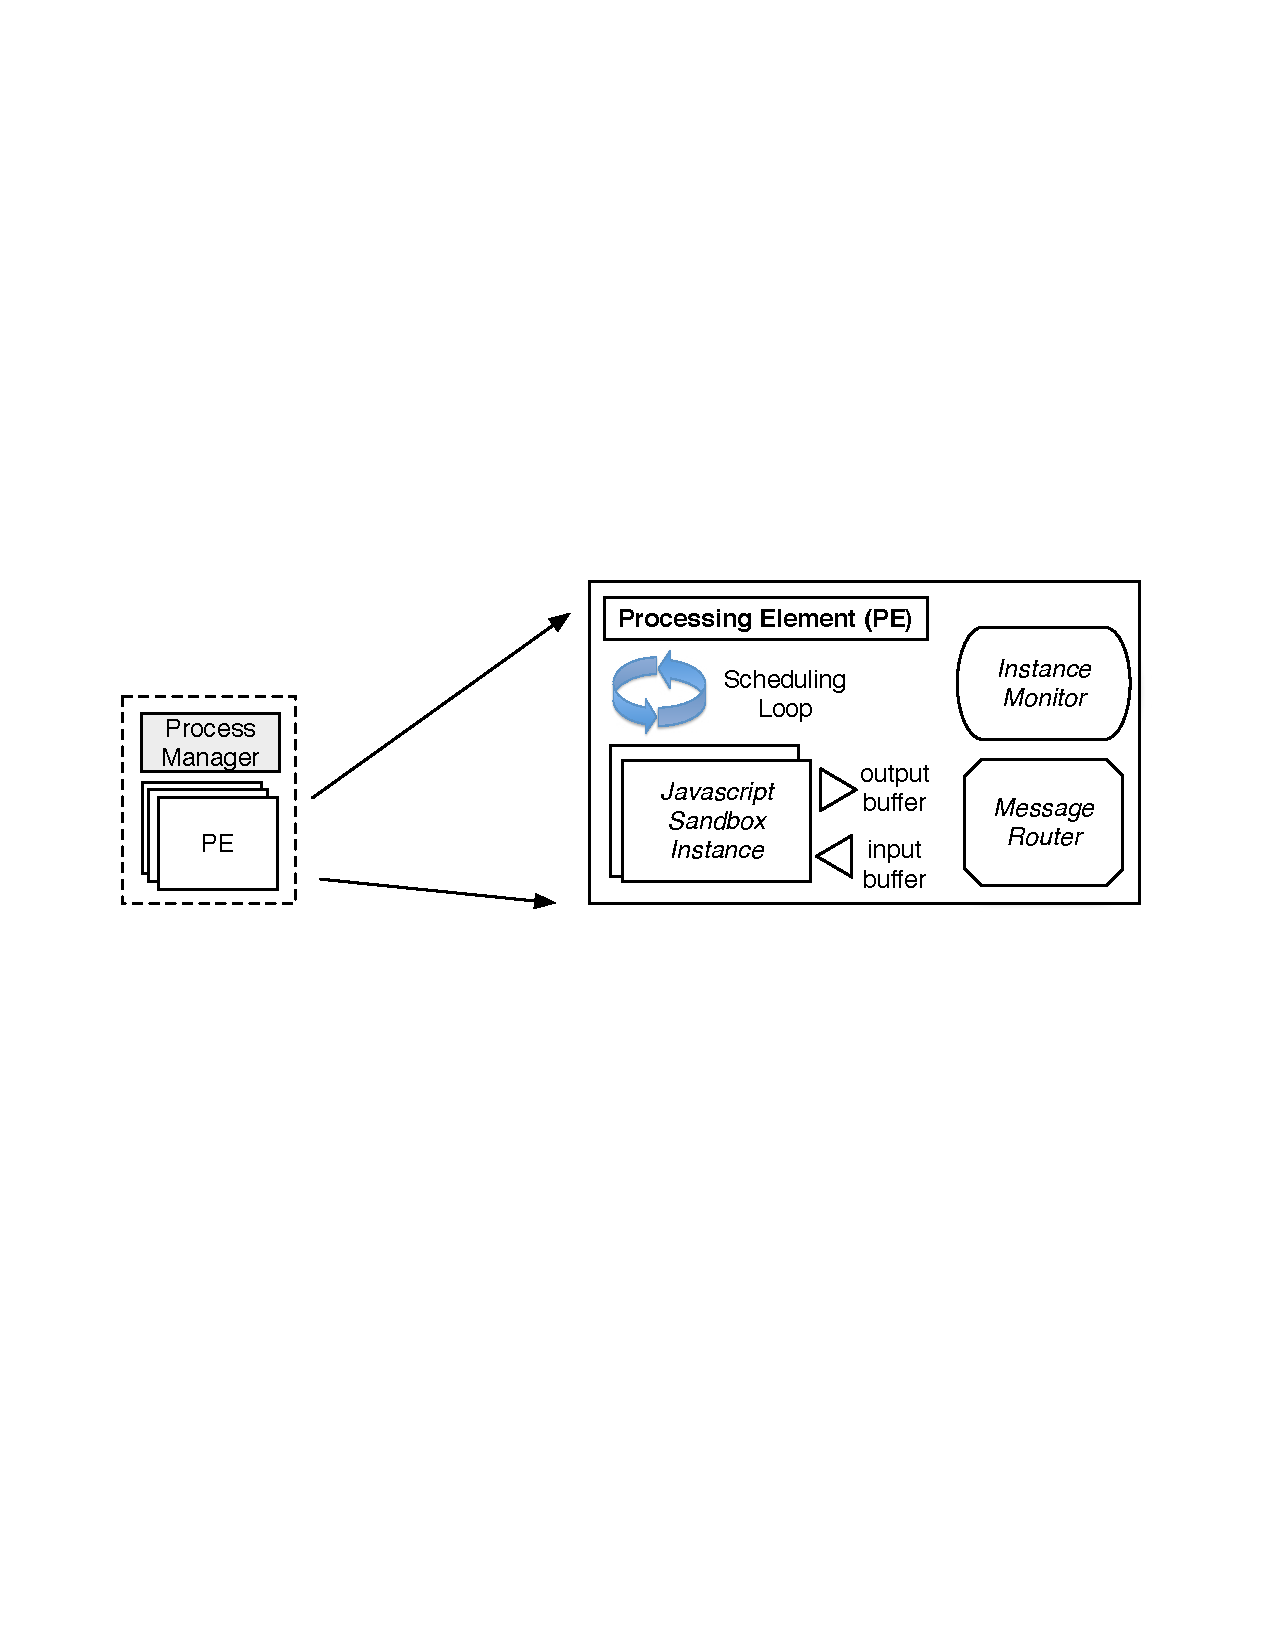
\includegraphics[width=0.85\columnwidth]{figs/pe_internals}
\caption{This figure shows the internal structure of a process element (PE).  The PE consists of several
javascript sandboxes where internal process code runs.  It also contains a scheduling loop, message router, and instance 
monitor.}
\label{fig:pe_internals}
\end{figure}


The process element stub that runs on a separate machine.  Its main job is to manage the jobs that are being executed on that
machine.  Figure~\ref{fig:pe_internals} shows the components of a process element.  There are four main components in the unit.

\begin{enumerate}
\item \emph{Scheduler}: The scheduler manages the execution schedule for each job running in a sandbox.  The scheduler uses
the \texttt{timeout} as the execution period of the job.

\item \emph{Sandbox}:  The sandbox is where the javascript code runs.  The sandbox contains an input and output buffer and simply 
waits for either an execution signal from the scheduler or until the input buffer has \texttt{window} element in it.  The output
buffer is of size 1.  The object returned by the job is written to the output buffer.

\item \emph{Message Router}:  The message router communicates with the process manager and sends control and data messages between
the PE and the process manager.  It monitors the output buffer for each of the elements and forwards them to the process manager 
when it is populated.

\item \emph{Instance Monitor}:  The instance monitor manages the state of the sandbox.  If a sandbox dies, the instance monitor re-starts
it.  If it continues to die, it kills the sandbox process and forwards an error message to the message handler to the process manager.
The process manager annotates the instance file with the error.

\end{enumerate}


The process manager keeps a map of which process elements own which jobs.  If a process element goes down, the jobs are automatically
migrated to another process element and the process element is removed from the active list.  Each PE and job have a unique identifier.
The messages received from the \emph{message router} in the PE are annotated with these ids and the process manager uses these
to update the associated instance file in StreamFS.  Again, everything is managed in through filesystem.  So errors and data
are exposed to external applications through the meta/data in the files.

Note, the process manager maintains a mapping between job instances and PEs.  It also notes the machine the PE is running on.  The
\emph{instance monitor} allows the process manager to make decisions about job migration in case of failure.  PEs are designed
to function independently from one another.  This allows the process cluster to scale linearly with the load -- in terms of
the number of streams being processed and the number of active jobs.  Like the other components in StreamFS, it is 
\emph{horizontally scalable}.  The process manager serves as a single point of failure.  If it fails it must be restarted manually.
Any messages sent from the PE to the process manager during the down period is lost.

% Our contributions are:  

% \begin{itemize}
% \item Use of the entity-relationship graph to provide OLAP \emph{roll-up}, \emph{drill-down},
%         and \emph{slice and dice} operations.
% \item Show how sliding-window operations can be used on real-time data in combination with the entity-relationship
%         graph to maintain accurate aggregates as the underlying objects and inter-relationships change.
% \end{itemize}

% \subsection{Mapping OLAP to ERG}
\subsection{OLAP-style Aggregation}

% \begin{itemize}
% \item Introduction to OLAP.
% \item Explanation of ERG in StreamFS.
% \end{itemize}
Online analytical processing (OLAP) provides summarization of data
from a set of underlying data repository (date warehouses).  Traditionally, OLAP is used to process
business data.  Business data summarization allows an analyst to ask targeted questions about aggregates 
and trends in their data.  The data is typically multidimensional in nature and operations can be performed with
respect to those dimensions and their inter-relationship.  In our deployments, we find that most queries are 
similar to OLAP queries with scan-heavy queries across the time dimension.

We introduce a mechanism that can perform hierarchical aggregates across a unit of measure, used in combination
with the timeseries data store to support scan-heavy queries, called \emph{aggregation points}.  We discuss
these in more detail in Section~\ref{sec:aggpts}.  However, before discussing aggregation points, we give details
on how we make use of the entity-relationship graph and timeseries database to support OLAP-style queries.

OLAP schemas logically construct a hypercube with different dimensions along each axis.  We presented a visual translation of
a OLAP cube to an entity relationship graph in Section~\ref{sec:erg2olap}.  Specifically, we showed in Figure~\ref{fig:olap2erg}
that each dimension is essentially a unit of measure, the hiearchy is explicitly constructed, and there
time is a dimension that is stored in a timeseries database.  We show how the terminology also translates and some
examples of certain classes of OLAP queries, how they are constructed, and how they are satisfied by StreamFS.

\subsubsection{Measures, Dimenions, and Levels}
\emph{Measures} refer to the actual value, located somewhere is the cube along the intersection of several dimensions.
A \emph{dimension} is simply a reading and an example is shown in Figure~\ref{fig:olap2erg}.  Dimensions 
are labels for an axis.  In StreamFS a measure is a unit of measure (i.e. Fahrenheit) or time.  The hierarchical \emph{level}
is explicit in the construction of the names.  So in the subtree that organizes streams according to the location of the
in space, the floor level would be above the room level.  These points can be designated as aggregation points, whereby
all streams that have the specified units, are aggregated at that point and the data are stored like any other streams.

\subsubsection{Operations: drill-down and roll-up}
Drill-down and roll-up are explicit in the structure.  You can drill down to individual readings or roll them
up into an aggregation point at a particular level in the hierarchy.  Essentially the level is an explicitly specified in the 
name of either the raw stream or the aggregation point.

\subsubsection{Operations: Slice and Dice}
Slice and dice queries are queries that either take a slice of the cube along a dimension or pick a sub-cube from the cube.
Slice and dice operations are translated as traversals of the hierarchical structure across levels and units.  Figure~\ref{fig:olapslice2ergslice}
shows how a slice query is satisfied on a hierarchical structure.  The corresponding slice query 
is \\ \texttt{query.slice('/4F/R*').start(t1).end(t2);}.

\begin{figure}[h!] %htbp
\centering
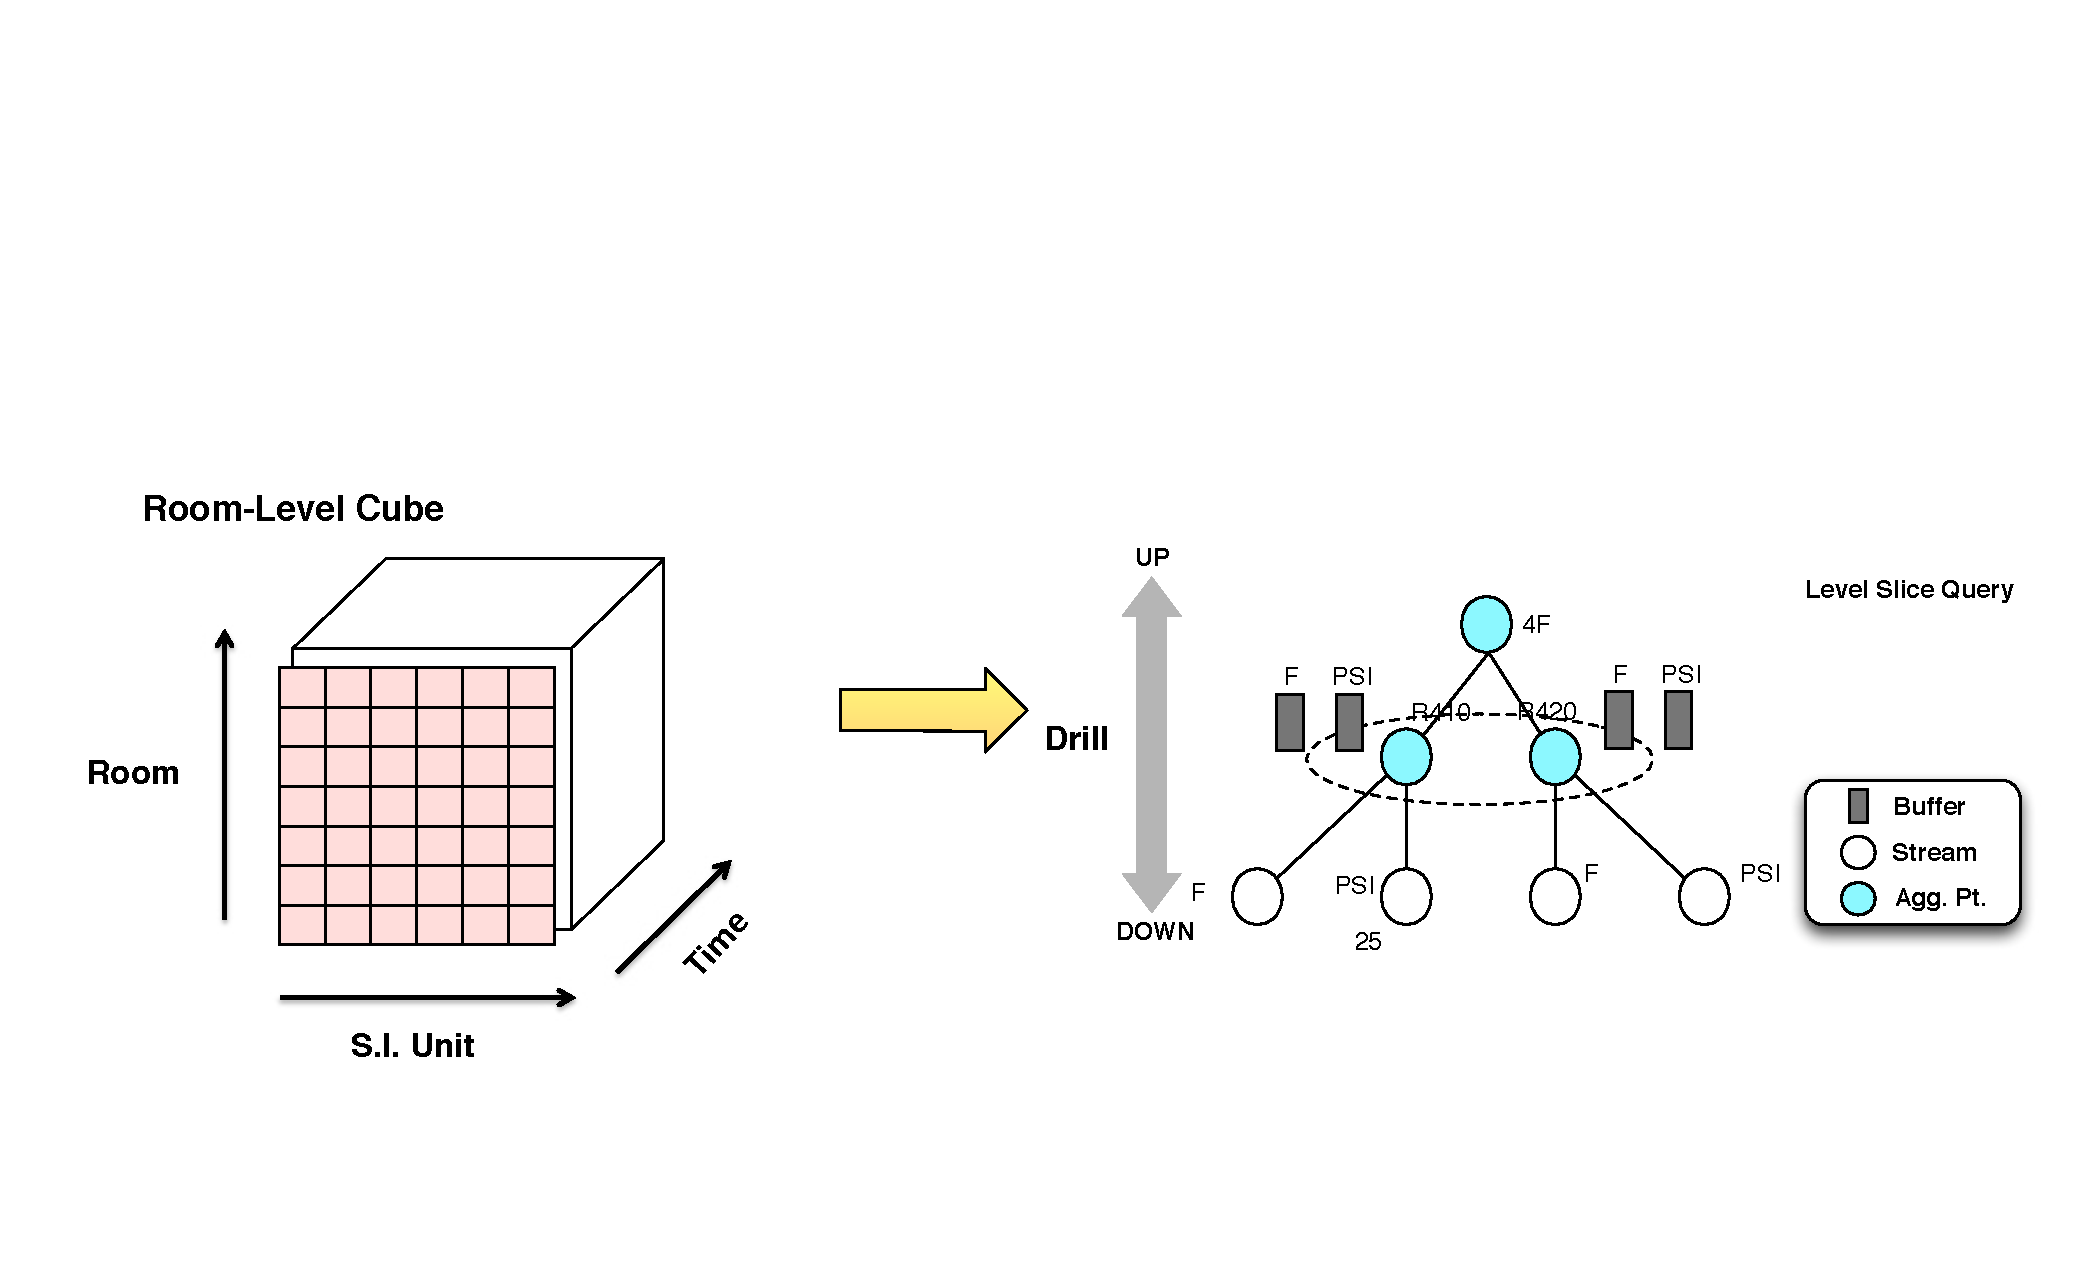
\includegraphics[width=1.0\columnwidth]{figs/olapslice2ergslice}
\caption{This figure shows how a ``slice'' operation is translated from the cube to the ERG.  The user queries across all streams or aggregation
points at a certain level, specified by a star level query with the level-specific prefix.  The corresponding slice query is
\texttt{query.slice('/4F/R*').start(t1).end(t2)}.
}
\label{fig:olapslice2ergslice}
\end{figure}


% \begin{lstlisting}[caption={Slice query example.},label={code:slice_query}]
% query.slice('/4F/R*').start(t1).end(t2);
% \end{lstlisting}

Figure~\ref{fig:olapdice2ergdice}
shows how a dice query is satisfied on a hierarchical structure.  The corresponding dice query 
is \texttt{query.dice('/4F/R*').units(['F']).start(t1).end();}.


\begin{figure}[h!] %htbp
\centering
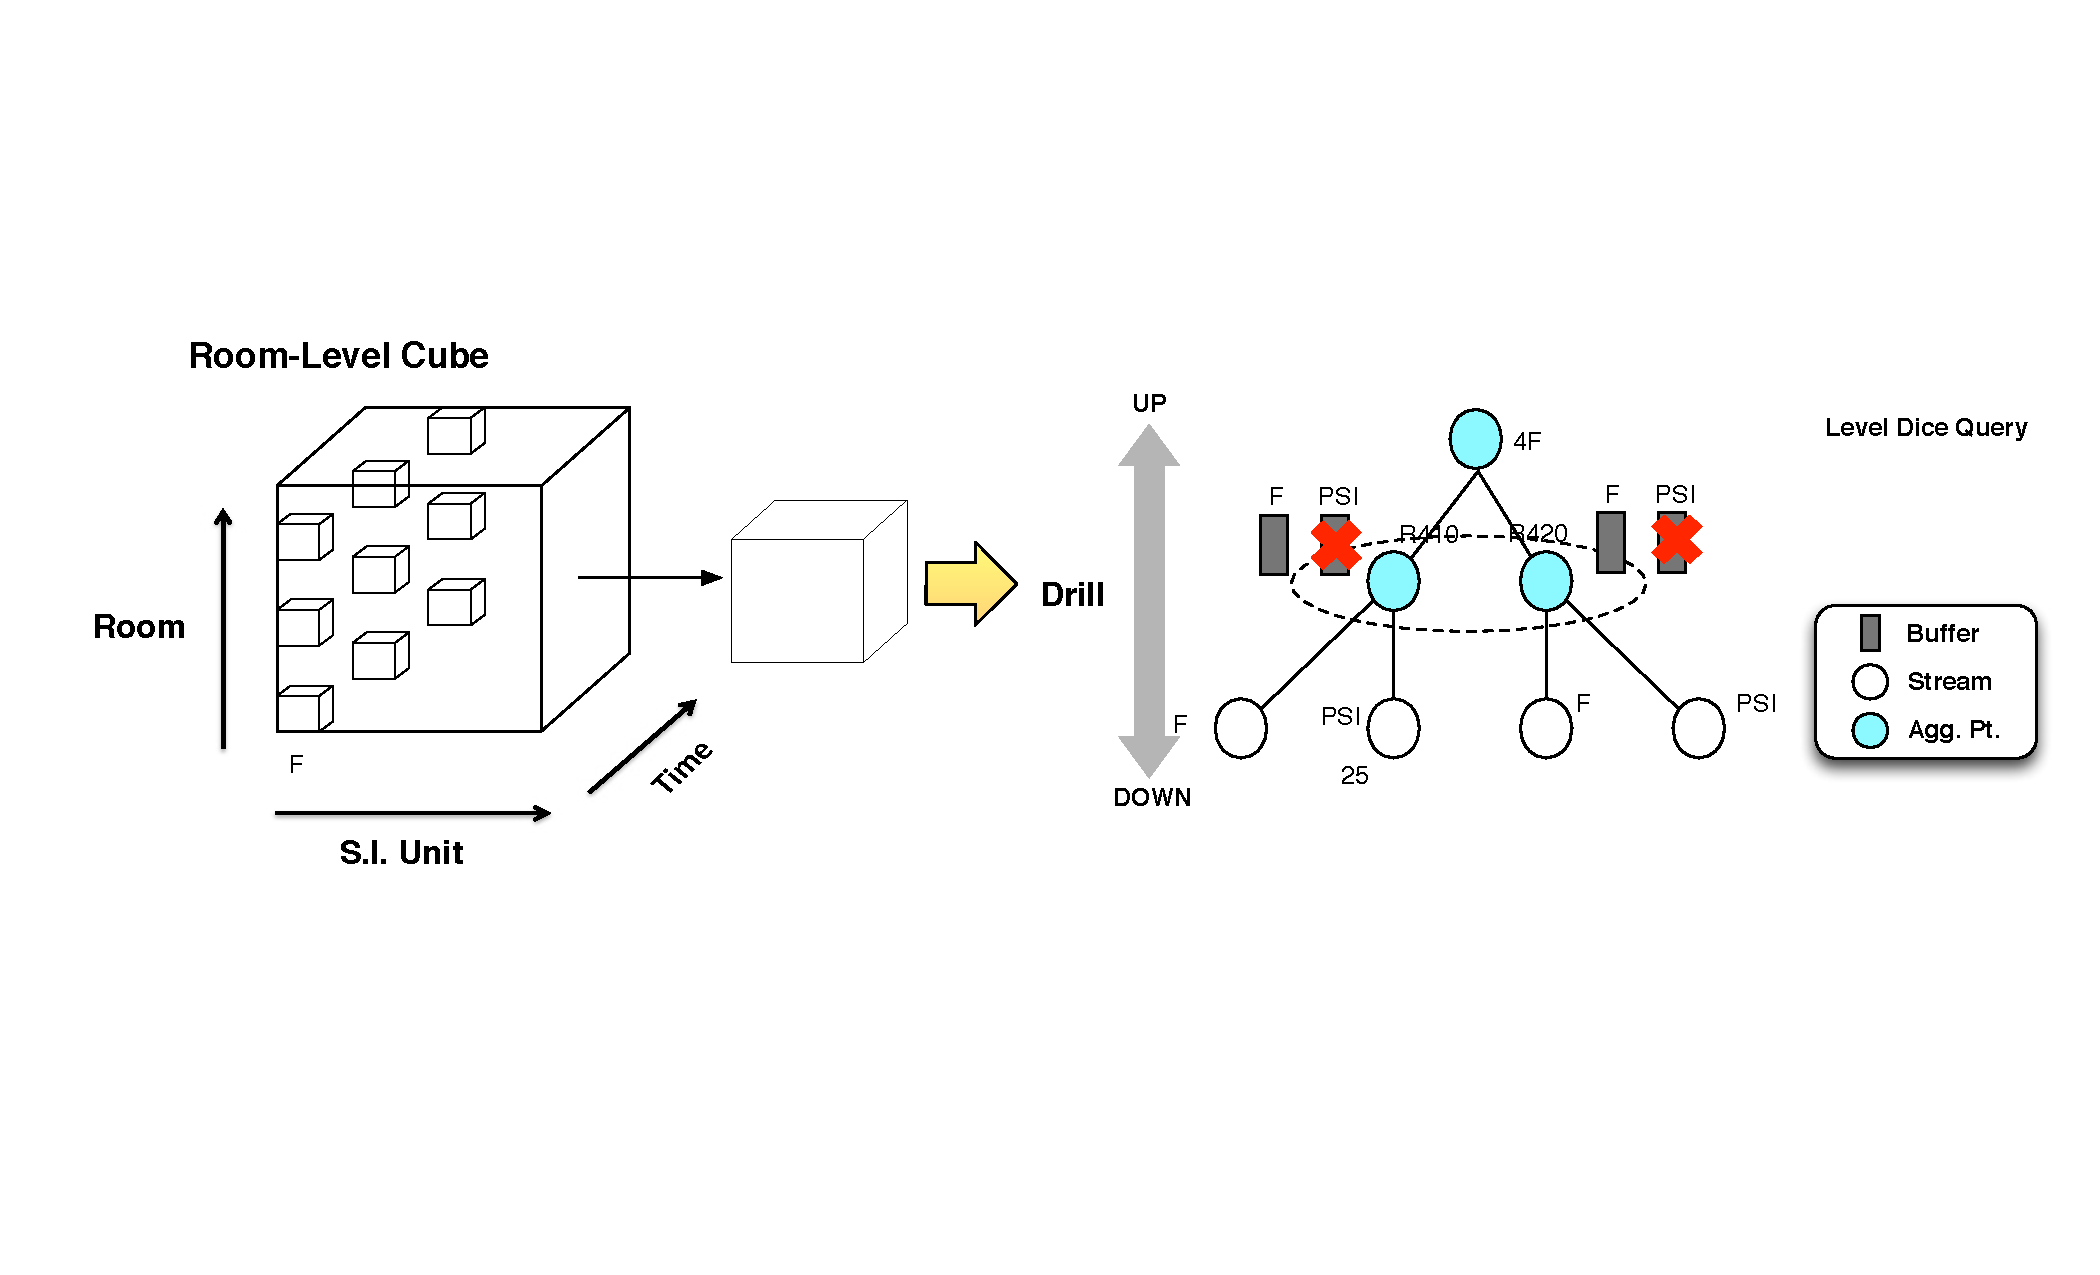
\includegraphics[width=1.0\columnwidth]{figs/olapdice2ergdice}
\caption{This figure shows how a ``dice'' operation is translated from the cube to the ERG.  The user queries across all streams or aggregation
points at a certain level, specified by a star level query with the level-specific prefix.  The corresponding dice query is
\texttt{query.dice('/4F/R*').units(['F']).start(t1).end()}.}
\label{fig:olapdice2ergdice}
\end{figure}


% \begin{lstlisting}[caption={Dice query example.},label={code:dice_query}]
% query.dice('/4F/R*').units(['F']).start(t1).end();
% \end{lstlisting}


\subsubsection{Operations: Pivot}
Pivot operations are not explicitly supported.  Although you can imagine that if you cut across a hierarchical level across all dimension, can
can effectively construct a pivot-style query.



\subsection{Aggregation Points}
\label{sec:aggpts}
StreamFS makes use of OLAP-style mechanism to provide the end-user with \emph{aggregation points} in the hierarchy.
StreamFS distinguishes between nodes that represent streaming data sources and those that do not.  Those that do not, 
however, can be tagged as aggregation points.  
% As part of the tagging processes, a user specifies the units of aggregation, with 
% additional options for cleaning and processing.  
When node is tagged as an aggregation point all the points root at that
node in the tree are set as aggregation points and all streams are aggregated and save to the timeseries database.
Since streams are not synchronized (i.e. they do not produce data at the same time) each time a value arrives from a
sensor the value for all other streams is interpolated and aggregated along the \emph{unit} level dimension.
%an example?

This propagates up to the aggregation point and all of it is saved in the timeseries database.  The aggregation function
can be specified by the user, with the default set to as \texttt{sum}.  Other options include \emph{avg, sum, max, min} and
a custom function that can be specified by the user. %pointer to an internal/external process definition file
% Aggregation points are also critical for support OLAP-style queries and \emph{dynamic aggregation}, discussed in
% the next two sections.

%FILL IN WITH REAL GRAPH
\begin{figure}[htb!]
\begin{center}
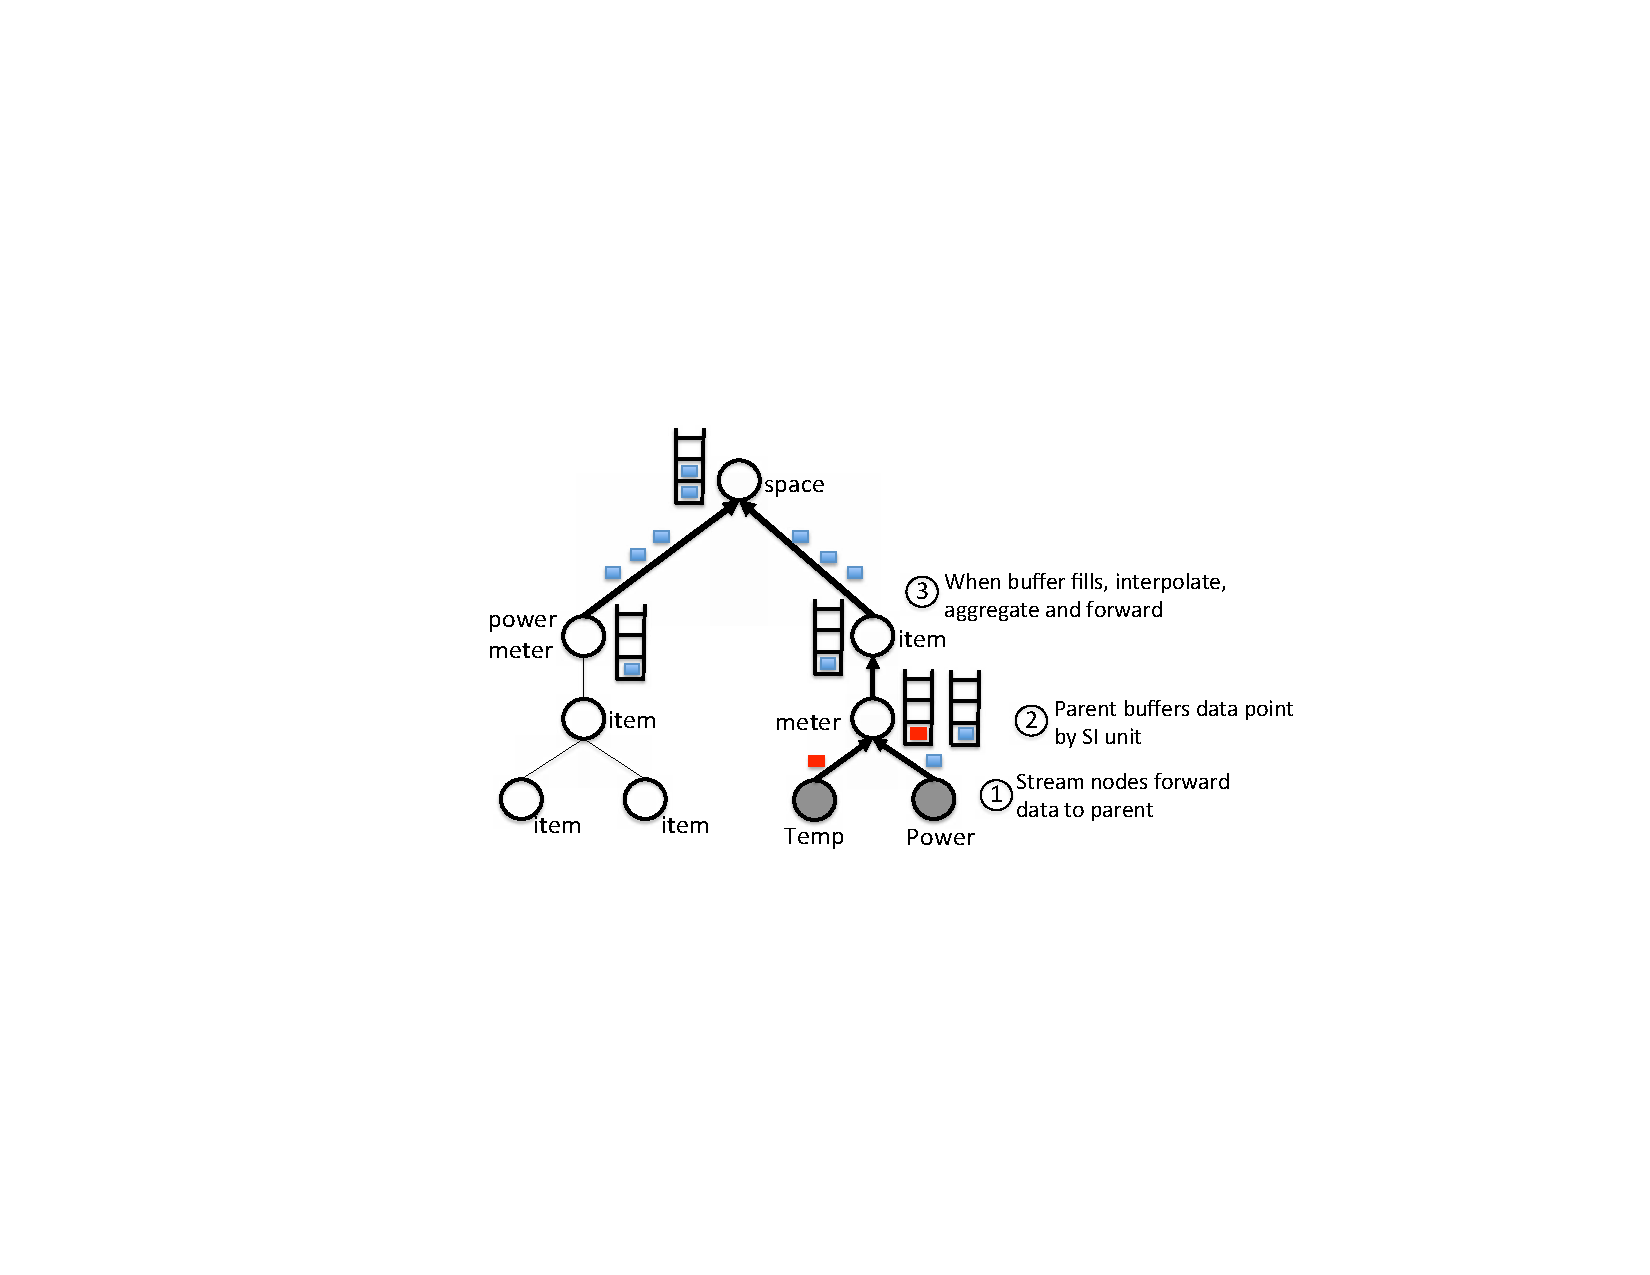
\includegraphics[scale=0.6]{figs/aggtree}
\caption{This shows an illustration of the aggregation tree used by \emph{dynamic aggregation}.  Data flows from 
the leaves to the root through user-specified aggregation points.  When the local buffer is full the streams
are separated by source, interpolated, and summed.  The aggregated signal is forward up the tree.}
\label{fig:aggtree}
\end{center}
\end{figure}

% Aggregation points combine the underlying entity-relationship graph with in-network aggregation.  It treats
% each node in the graph as a potential point of aggregation on a particular data type.  
Consider the following example.  We need to compute aggregates of \emph{KW} data and we declare the node for a particular room as
the point of aggregation, we accept data from all children of that node that, whose units are in \emph{KW},
and add the streams together over pre-defined window size or pre-defined timeouts.

The scheme is hierarchical, so a node only accepts data from its children and only sends data to its parent.
StreamFS checks for cycles when before node insertion and prevents double-counting errors by only allowing 
aggregation-points that are roots of a tree that is a sub-graph of the entity-relationship graph.  In our deployment,
each view is a managed as an independent hierarchy.  So the hierarchy of \emph{spaces} is separate from
the \emph{inventory} hierarchy or the \emph{taxonomy} hierarchy.  This allows us to ask questions with a particular
view in mind, without conflict, and is a natural fit for our aggregation scheme.

% \subsubsection{How it works}
Although there are different semantics applied to different file types at the application layer, dynamic aggregation
mainly deals with two types of files: (1) container nodes and (2) stream nodes.  The main difference is that \emph{container} nodes
are not explicitly associated with data coming from a sensor and \emph{stream} nodes are.  Furthermore, container
nodes can have children, while stream nodes cannot.  In our application, meters are represented by container nodes
and each stream of data they produce is a stream node.

When an aggregation point is enabled, dynamic aggregation places a buffer at the node for the type
of data that should be aggregated.  
If we want to aggregate \emph{KW} data, we specify the type and send an enable-aggregation
request to StreamFS.
% to the node through an HTTP {\texttt POST} to the path for that node.  
The flow of data starts at the leaves when
a stream node receives data from a sensor.% through HTTP {\texttt POST}.  
As data arrives it is immediately
forwarded upstream to the parent(s).  
% If a node that receives data from its children is an aggregation point it buffers
% the data, otherwise it forwards it to its parent.

Ignoring the timeouts for now, lets imagine the parent is a point of aggregation and its buffer is full.  At this point
the parent separates data into bins for each source and cleans it for aggregation through interpolation.  The main
operation is to \emph{stretch} and \emph{fill} that data with linearly interpolated values.  The \emph{stretch}
operation orders all the timestamps in increasing order and, for each bin, interpolates the values using the
first (last) pair of data points.  If there is only a single data point, the stretch uses it as the missing value.
The \emph{fill} operation find the nearest timestamps that are less-than and greater-than the missing sampling time, 
uses their values to determine the equation of a line between them and interpolates the missing value using that equation.
Once this is done for each signal, the values are added together for each unique timestamp and the aggregated
signal is reported to the parent, where the operation occurs recursively to the root.
Figure~\ref{fig:aggtree} shows an illustration of this processing structure.


% \subsection{Dynamic Aggregation}


%problem:  the buffer size has to increase exponentially up the tree, in order to not drop any values.
%solution: chuck the data into default-buffer sized pieces and parallelize the interpolation using the interpolated tasks technique




\subsubsection{Dealing with dynamics}
\label{sec:dynagg}

This approach deals with changes in the graph quite naturally.  All aggregation points deal only with local data, so
a node is only concerned about the children that give it data and the parent to send data to.  As objects in the environment
move from place to place and these changes are captured, the entity-relationship graph also changes to reflect the move.
This change in aggregation constituents is naturally accounted for in the aggregate.  Since the underlying pub-sub mechanism
drives the forwarding (see Section~\ref{sec:ProcMngtSchedMain}) the removal of a child will reject any new data that comes 
in for the removed node.  As such, it will
not be accounted for in the aggregate.  If a new child is added, it is forwarded up the tree, since the name associated
with the data point will indicate its position in the hierarchy.
% When a child is removed,
% it no longer forwards data to the old parent, therefore the aggregate will reflect that change.
Note, however, that changes in the entity-relationship graph are indistinguishable from energy-consuming items that have
been turned off.  For the purposes of aggregation, that is okay.

OLAP-style aggregation is an expensive feature.  Each point in the subtree rooted at the aggregation point is automatically
activated to produce streaming data.  Special internal processing elements are enabled to compute the aggregates and run
the pre-processing and communication between the processing unit and name server increases as data is returned from the 
process elements to be routed to the timeseries data store.  The amount of processing and storage scales linearly with the 
number of streams and the number of aggregation points in the sub-tree.



% For demonstration lets have the user turn off on of their appliances when they leave as well.  This should cause that total
% room aggregate to drop, the person's personal aggregate to drop, but the other occupant's aggregate to remain
% the same.

% %FILL IN WITH REAL GRAPH
% \begin{figure}[htb!]
% \begin{center}
% 
\includegraphics[scale=0.39]{figs/blankbox}
% \caption{A room with items that belong to many users.  Person leaves with their item, aggregate falls.  Show aggregate.
% Person joins another room, aggregate in that room rises.  Show aggregate in the new room.  Compare before and after.}
% \label{fig:personaltotalagg}
% \end{center}
% \end{figure}

% Figure~\ref{fig:personaltotalagg} illustrate the results of the second scenario.  Note how...

